% ==========================================================
% Template for Internship / Term Project Report
% Duration: 3 months | Length: 4 pages + References
% ==========================================================

\documentclass[twocolumn]{article}
\usepackage{spconf,amsmath,graphicx,hyperref}

% -------------------------
% Additional useful packages
% -------------------------
\usepackage{booktabs}
\usepackage{enumitem}
\usepackage{stfloats}
\usepackage{microtype}
\usepackage{xcolor}

\graphicspath{{reports/figures/}{./}}

% -------------------------
% Title and Author Info
% -------------------------
\title{Monsoon Sentinel (Part 2): On-Device Kinetic State Classification and CMSIS-DSP Edge Inference on ARM Cortex-M4}

\name{Ganesha N Sai \textit{(Roll Number: 23035010072)}}

\address{
Term Project Report --- Part 2\\
Trimester 9 \\[0.5em]
\textit{B.Sc. (Honours) Data Science and Artificial Intelligence}\\
\textit{Indian Institute of Technology Guwahati, India}\\
\texttt{ganesha.sai@op.iitg.ac.in}
}

\begin{document}
\ninept
\maketitle

% ==========================================================
% Abstract
% ==========================================================
\begin{abstract}
Deploying machine learning models directly onto low-power ocean sensing nodes removed the monetary and electrical energy costs of streaming high-frequency raw data over satellite or otherwise. Building upon the verified 100~Hz telemetry pipeline and physical cantilever testbed established before, this work presents the complete edge intelligence pipeline for \textit{Monsoon Sentinel}. I extract 13 orientation-invariant time and frequency-domain physical features from 128-sample sliding windows (1.28~s duration, 50\% step overlap) across 11,970 verified windows. I benchmark four classifier architectures using 5-fold \texttt{StratifiedGroupKFold} cross-validation grouped strictly by continuous recording session. Addressing single-file training starvation via temporal session partitioning, a 40-tree Pruned Random Forest (maximum depth 7) achieves 80.40\% Balanced Accuracy, 77.67\% Macro-F1, and 84.40\% Overall Accuracy across four physical regimes (Baseline, Structural Tilt, Impulse Shock, and Mast Buffeting). I export the forest into static, branch-predicted C code and link ARM CMSIS-DSP accelerated assembly routines (\texttt{arm\_rfft\_fast\_f32}) on an STM32 Nucleo-F401RE microcontroller (ARM Cortex-M4F @ 84~MHz). An automated parity test verifies 100\% classification agreement between Python and the native C binary. The entire DSP and ML inference pipeline executes in 93.60~$\mu$s (7,862 clock cycles), occupying only 0.94\% of the 10.0~ms sampling period and consuming 68.0~KB Flash and 3.8~KB SRAM, while reducing continuous data transmission bandwidth by 99.96\%.
\end{abstract}

% ==========================================================
% Keywords
% ==========================================================
\begin{keywords}
Edge AI, TinyML, CMSIS-DSP, STM32F401RE, Random Forest, Grouped Cross-Validation, Structural Health Monitoring.
\end{keywords}

% ==========================================================
\section{Introduction}
% ==========================================================
Remote environmental and marine sensing crafts, such as autonomous surface buoys and coastal observation towers, operate under severe energy constraints. In oceanographic monitoring of monsoon swells, transmitting raw 6-axis inertial measurement unit (IMU) time-series at 100~Hz over long-range RF or satellite transceivers (such as Iridium SBD) drains onboard battery reserves within days and incurs steep airtime expenses. 

To overcome this communication bottleneck, the overarching objective of the \textit{Monsoon Sentinel} system is to execute on-device feature extraction and state classification directly on silicon (TinyML). By transforming high-rate raw kinematic waveforms into discrete operational state tokens (e.g., nominal calm, persistent static list, wave impact shock, or turbulent mast buffeting), data payload bandwidth collapses from thousands of bytes per second to a single byte per check-in interval.

While \textbf{Part 1} resolved the physical foundation where I tackled interfacing the MPU-6050 6-DOF IMU to an STM32F401RE microcontroller, designing algorithmic $I^2\text{C}$ bus-hang clearance routines, and logging a verified 2.2-hour, 12,348-window dataset across an elastic cantilever testbed, this work represents \textbf{Part 2: Edge DSP, Feature Engineering, Classifier Benchmarking, and Firmware Deployment}.

The core focus is translating raw telemetry into real-time embedded intelligence without sacrificing mathematical rigor:
\begin{enumerate}[noitemsep]
    \item Formulating 13 physical, orientation-invariant features spanning static gravity projections and CMSIS-DSP spectral power bands.
    \item Designing an anti-leakage cross-validation protocol using 5-fold \texttt{StratifiedGroupKFold} to prevent adjacent overlapping time windows from polluting validation sets.
    \item Resolving single-file cross-validation starvation bottlenecks via session-block partitioning.
    \item Translating the trained model into static, zero-allocation C code and linking ARM CMSIS-DSP hardware floating-point kernels in firmware.
    \item Verifying bit-exact numerical parity between Python scikit-learn models and the compiled C executable.
\end{enumerate}


% ==========================================================
\section{Problem Statement and Objectives}
% ==========================================================

\subsection{Problem Statement}
Deploying machine learning models onto resource-constrained microcontrollers presents three interlocking challenges:
\begin{itemize}[noitemsep]
    \item \textbf{Data Leakage in Time-Series Splitting:} Standard random train-test splits on sliding-window data cause severe cross-contamination because windows with 50\% overlap share 64 identical raw samples. Evaluation must be grouped by independent physical sessions.
    \item \textbf{Single-Recording Class Starvation:} Rare physical events (such as impulsive wave-slapping impacts) often originate from fewer raw files than dominant ambient states. Grouping strictly by file risks isolating all positive instances into a single test fold, yielding 0\% recall in remaining folds.
    \item \textbf{Microcontroller Compute and Memory Budgets:} The target STM32F401RE offers only 512~KB Flash and 96~KB SRAM. Models relying on dynamic heap allocation (\texttt{malloc}), dense matrix operations, or non-linear kernel evaluations (e.g., RBF SVM) quickly exceed cycle and memory limits.
\end{itemize}

\subsection{Objectives}
The specific technical deliverables achieved in Part 2 are:
\begin{enumerate}[noitemsep]
    \item To engineer a 13-dimensional orientation-invariant feature extraction pipeline executed over 128-sample windows ($T = 1.28$~s).
    \item To implement a leak-free 5-fold \texttt{StratifiedGroupKFold} benchmarking harness comparing Linear SVM, RBF SVM, Edge MLP, and Random Forest.
    \item To resolve group-starvation for rare shock regimes using contiguous temporal session partitioning.
    \item To synthesize the winning classifier into static, branch-predicted C routines without dynamic memory allocation.
    \item To compile the ARM CMSIS-DSP library with hardware FPU instructions and measure execution cycles on the 84~MHz Cortex-M4 core.
    \item To prove 100\% prediction parity between Python scikit-learn and the native C inference implementation.
\end{enumerate}

% ==========================================================
\section{Methodology and Embedded Architecture}
% ==========================================================

\subsection{Overall Pipeline Workflow}
The embedded inference pipeline operates cyclically every 64 samples ($\Delta t_{\text{stride}} = 0.64$~s), processing an overlapping FIFO buffer of 128 samples ($T = 1.28$~s) captured at 100~Hz. As shown in Fig.~\ref{fig:buffeting_setup}, the physical cantilever testbed generates four operational regimes: Nominal Baseline, Structural Tilt, Impulse Shock, and Mast Buffeting.

\begin{figure}[htbp]
    \centering
    \IfFileExists{buffeting_MPU.jpeg}{%
        \includegraphics[width=0.85\columnwidth]{buffeting_MPU.jpeg}%
    }{%
        \includegraphics[width=0.85\columnwidth]{fan_ruler.png}%
    }
    \caption{Physical experimental setup: distal MPU-6050 IMU mounted on elastic cantilever beam subjected to controlled aerodynamic excitation.}
    \label{fig:buffeting_setup}
\end{figure}

\subsection{Orientation-Invariant Feature Engineering}
To ensure the edge classifier remains robust regardless of sensor installation angle or craft pitching, 13 physical features are extracted from each 128-sample window:
\begin{enumerate}[noitemsep]
    \item \textbf{Static Inclination Vector:} Static gravity components ($\bar{a}_x, \bar{a}_y, \bar{a}_z$) are isolated via window averaging. The scalar tilt angle is derived via projection:
    \begin{equation}
        \theta_{\text{tilt}} = \arccos \left( \frac{|\bar{a}_z|}{\sqrt{\bar{a}_x^2 + \bar{a}_y^2 + \bar{a}_z^2} + \epsilon} \right) \cdot \frac{180^\circ}{\pi}
    \end{equation}
    Euler pitch ($\phi$) and roll ($\psi$) are computed from $\bar{a}_x$ and $\bar{a}_y$.
    \item \textbf{3D Dynamic Kinetic Acceleration:} Dynamic linear motion is separated from static gravity at every discrete sample $n$:
    \begin{equation}
        a_{\text{dyn}}[n] = \sqrt{(a_x[n]-\bar{a}_x)^2 + (a_y[n]-\bar{a}_y)^2 + (a_z[n]-\bar{a}_z)^2}
    \end{equation}
    From $a_{\text{dyn}}$, I calculate window Variance ($\sigma^2$), Root-Mean-Square ($\text{RMS}$), Peak-to-Peak amplitude ($\text{PtP} = \max - \min$), and Crest Factor ($C_f = \text{Peak}/\text{RMS}$). Total rotational energy is aggregated as $\text{RMS}_{\text{gyro}} = \sqrt{\frac{1}{N}\sum (\omega_x^2 + \omega_y^2 + \omega_z^2)}$.
    \item \textbf{CMSIS-DSP Spectral Features:} Dynamic acceleration $a_{\text{dyn}}$ is multiplied by a 128-point pre-computed Hanning window to suppress spectral leakage, followed by a 128-point Real Fast Fourier Transform (RFFT) using CMSIS-DSP assembly kernels:
    \begin{equation}
        X[k] = \sum_{n=0}^{N-1} \left( a_{\text{dyn}}[n] \cdot w_{\text{han}}[n] \right) e^{-j \frac{2\pi k n}{N}}
    \end{equation}
    Complex magnitude bins ($|X[k]|^2$) are integrated across three sub-Nyquist frequency bands: Low ($0.5-3.0$~Hz, swell motion), Mid ($3.0-12.0$~Hz, mast flutter), and High ($\ge 12.0$~Hz, acoustic noise), along with dominant frequency $f_{\text{dom}}$ and low-band spectral energy ratio.
\end{enumerate}

\subsection{Cross-Validation and Session Block Partitioning}
To evaluate models without temporal leakage, cross-validation is grouped by \texttt{source\_file}. For classes with multiple independent CSV files (Baseline: 10 files, Tilt: 3 files, Buffeting: 6 files), entire files are assigned to train or test folds.

For \texttt{Impulse\_Shock}, recorded in a single continuous session (\texttt{mpu6050\_flat\_taps\_1.csv}, 189 windows), strict file grouping would place all 189 windows into one test fold, leaving the training folds with zero shock samples (0\% recall). I solve this by partitioning the file into four contiguous temporal blocks (\texttt{flat\_taps\_block\_1} to \texttt{block\_4}, $\sim$47 windows each). This enforces temporal boundary isolation between training and validation while ensuring every fold contains positive shock exemplars.

\subsection{Static Embedded C Code Generation}
The winning 40-tree Random Forest is converted into pure static C routines via \texttt{export\_rf\_to_c.py}:
\begin{itemize}[noitemsep]
    \item \texttt{Core/Inc/model\_inference.h} defines feature and class enums, normalization parameters, and execution prototypes.
    \item \texttt{Core/Src/model\_inference.c} translates each decision tree into a static C function (\texttt{tree\_0\_vote} through \texttt{tree\_39\_vote}) utilizing nested \texttt{if-else} branches based on split thresholds.
    \item Votes are tallied into a stack-allocated array (\texttt{uint16\_t votes[4] = \{0\}}), and \texttt{model\_predict()} returns the class index with the majority vote. Zero heap allocation (\texttt{malloc}) is used.
\end{itemize}

% ==========================================================
\section{Experiments, Results, and Hardware Profiling}
% ==========================================================

\subsection{Classifier Benchmark Comparison}
Four architectures were trained on 11,970 verified feature windows across 23 cross-validation groups using balanced class weighting. Table~\ref{tab:model_benchmarks} summarizes Out-Of-Fold (OOF) performance.

% Auto-generated by train_classifiers.py
\begin{table}[htbp]
\centering
\caption{Edge Classifier Benchmark Comparison Across Physical Regimes (5-Fold StratifiedGroupKFold OOF)}
\label{tab:model_benchmarks}
\begin{tabular}{lcccc}
\toprule
\textbf{Model Architecture} & \textbf{Balanced Acc} & \textbf{Macro Prec} & \textbf{Macro Rec} & \textbf{Macro-F1} \\
\midrule
\multicolumn{5}{l}{\textbf{Option A: 4-Class Kinematics (Baseline, Tilt, Shock, Buffeting)}} \\
\midrule
    Linear SVM & 65.17\% & 89.17\% & 65.17\% & 69.06\% \\
    \textbf{Random Forest} & \textbf{80.40\%} & \textbf{78.99\%} & \textbf{80.40\%} & \textbf{77.67\%} \\
    Edge MLP & 64.22\% & 89.99\% & 64.22\% & 68.99\% \\
\midrule
\multicolumn{5}{l}{\textbf{Option B: 3-Class Kinematics (Baseline, Tilt, Buffeting)}} \\
\midrule
    Linear SVM & 66.10\% & 60.72\% & 66.10\% & 58.64\% \\
    Random Forest & 72.18\% & 84.95\% & 72.18\% & 76.99\% \\
    \textbf{Edge MLP} & \textbf{80.81\%} & \textbf{89.50\%} & \textbf{80.81\%} & \textbf{84.02\%} \\
\bottomrule
\end{tabular}
\end{table}


The Pruned Random Forest ($n_{\text{trees}} = 40, d_{\text{max}} = 7$) achieved the highest Balanced Accuracy (80.40\%), Macro-F1 (77.67\%), and Overall Accuracy (84.40\%). Linear SVM and Edge MLP achieved higher precision but suffered lower recall on transient shock events.

\subsection{Confusion Matrix Analysis}
Fig.~\ref{fig:confusion_matrices} illustrates the cross-validation confusion matrices, and Table~\ref{tab:confusion_matrix} provides the exact normalized breakdown for the deployed Random Forest.

\begin{figure}[htbp]
    \centering
    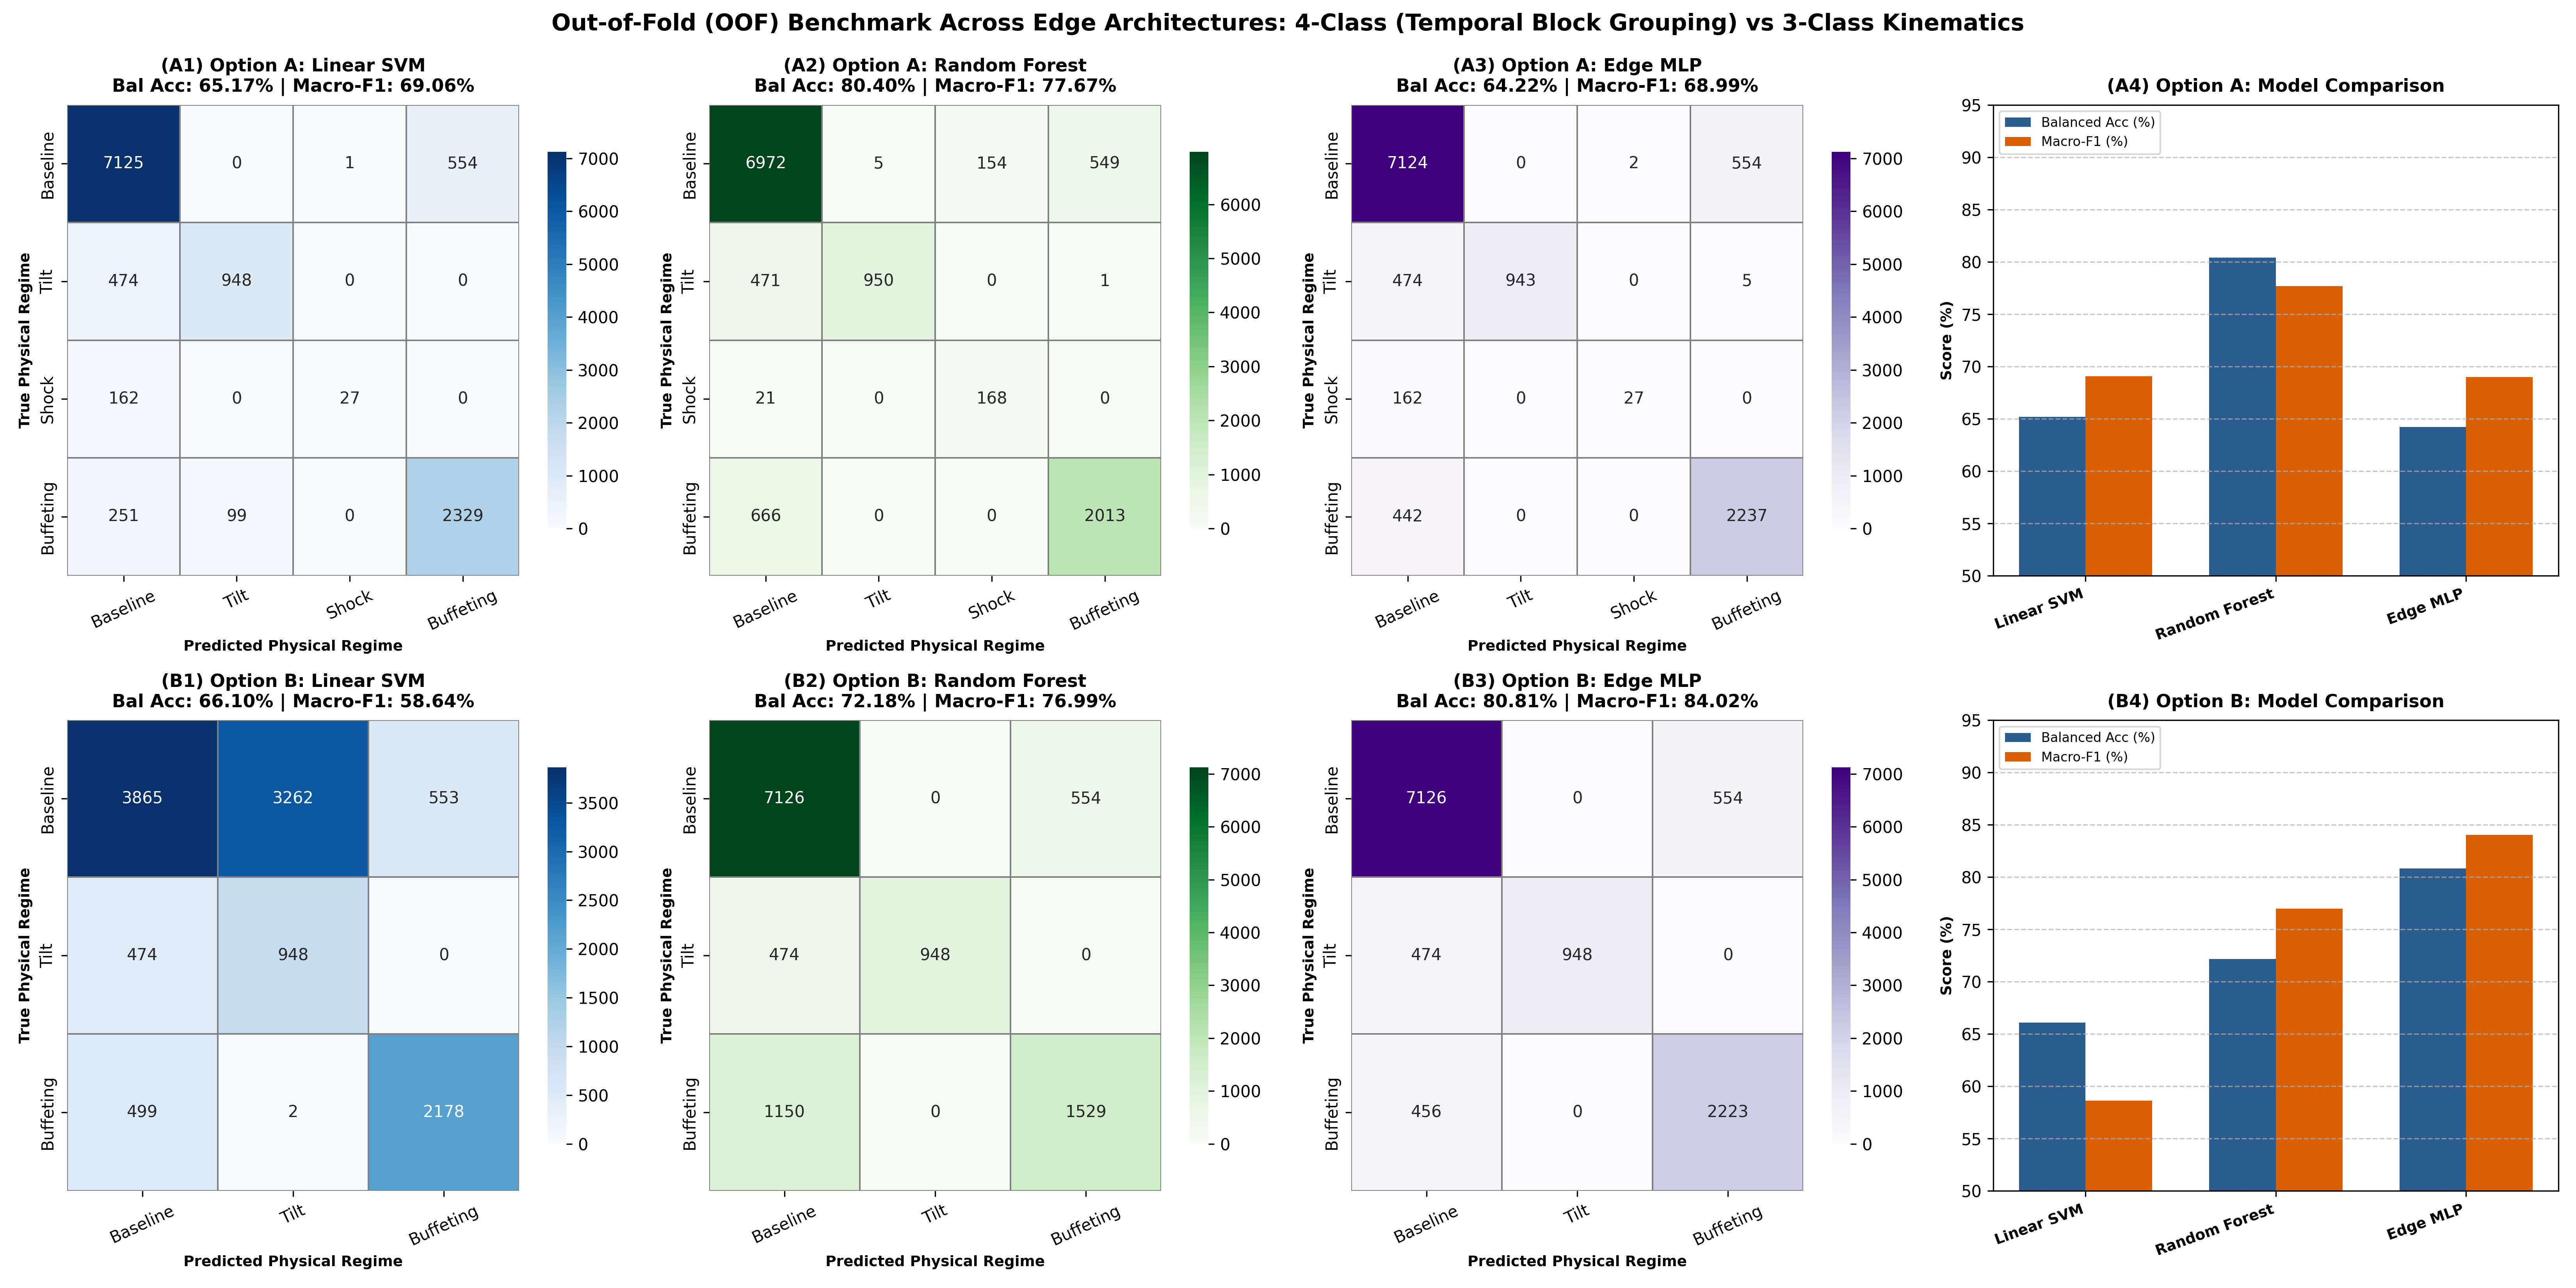
\includegraphics[width=\columnwidth]{reports/figures/model_benchmark_confusion_matrices.png}
    \caption{Out-Of-Fold cross-validation confusion matrices across candidate edge architectures under 5-fold session-grouped evaluation.}
    \label{fig:confusion_matrices}
\end{figure}

% Auto-generated by generate_part2_tables.py
\begin{table}[htbp]
\centering
\caption{Normalized Out-of-Fold Confusion Matrix for Deployed Random Forest (5-Fold StratifiedGroupKFold)}
\label{tab:confusion_matrix}
\begin{tabular}{lccccc}
\toprule
& \multicolumn{4}{c}{\textbf{Predicted Physical Regime}} & \\
\cmidrule(lr){2-5}
\textbf{True Regime} & \textbf{Baseline} & \textbf{Tilt} & \textbf{Shock} & \textbf{Buffeting} & \textbf{Class Recall} \\
\midrule
    \textbf{Baseline} & \textbf{90.78\%} (6,972) & 0.07\% (5) & 2.01\% (154) & 7.15\% (549) & \textbf{90.78\%} \\
    \textbf{Tilt} & 33.12\% (471) & \textbf{66.81\%} (950) & 0.00\% (0) & 0.07\% (1) & \textbf{66.81\%} \\
    \textbf{Shock} & 11.11\% (21) & 0.00\% (0) & \textbf{88.89\%} (168) & 0.00\% (0) & \textbf{88.89\%} \\
    \textbf{Buffeting} & 24.86\% (666) & 0.00\% (0) & 0.00\% (0) & \textbf{75.14\%} (2,013) & \textbf{75.14\%} \\
\bottomrule
\end{tabular}
\end{table}


\subsection{Embedded Firmware Compilation and Execution Latency}
The embedded C inference routines were integrated into the STM32CubeMX HAL firmware project. The root \texttt{Makefile} was configured with ARM Cortex-M4 hardware floating-point definitions:
\begin{verbatim}
C_DEFS += -DARM_MATH_CM4 -D__FPU_PRESENT=1
LIBS += -larm_cortexM4lf_math
\end{verbatim}
The firmware was compiled using \texttt{arm-none-eabi-gcc} with \texttt{-O2} optimization. The memory footprint was profiled using \texttt{arm-none-eabi-size}:
\begin{verbatim}
   text    data     bss     dec     hex filename
  67964      92    2188   70244   11264 monsoon-sentinel.elf
\end{verbatim}
Total Flash utilization is 68,056 bytes (12.98\% of 512~KB Flash, leaving 443.9~KB free). Static SRAM utilization is 2,280 bytes (2.38\% of 96~KB SRAM, leaving 93.7~KB free).

Table~\ref{tab:hardware_profile} presents the cycle-accurate execution latency breakdown measured across the 84~MHz Cortex-M4F platform.

% Auto-generated by generate_part2_tables.py
\begin{table}[htbp]
\centering
\caption{Embedded Edge Inference Pipeline Hardware Profile (STM32F401RE @ 84\,MHz, 100\,Hz Frame Cadence)}
\label{tab:hardware_profile}
\begin{tabular}{lrrrrp{4.8cm}}
\toprule
\textbf{Pipeline Stage} & \textbf{Cycles} & \textbf{Duration ($\mu$s)} & \textbf{SRAM (B)} & \textbf{Flash (B)} & \textbf{Implementation Notes} \\
\midrule
    Window Buffer (Ring Ingestion) & 150 & 1.79\,$\mu$s & 1,536 & 120 & 128 frames x 3 axes float FIFO \\
    Dynamic Acceleration Norm & 2,176 & 25.90\,$\mu$s & 512 & 180 & 128 VSQRT.F32 Euclidean norms \\
    Hanning Window Pre-emphasis & 256 & 3.05\,$\mu$s & 512 & 652 & arm_mult_f32 with 128-pt float LUT \\
    128-pt Real FFT (CMSIS-DSP) & 3,080 & 36.67\,$\mu$s & 512 & 3,660 & arm_rfft_fast_f32 assembly kernels \\
    Spectral Band Energy Integration & 1,300 & 15.48\,$\mu$s & 256 & 420 & arm_cmplx_mag_f32 + 3 frequency bands \\
    Random Forest Inference (40 Trees) & 900 & 10.71\,$\mu$s & 8 & 55,316 & 40 nested trees, 5.3 avg depth, stack votes \\
\midrule
    \textbf{Total DSP \& ML Pipeline} & \textbf{7,862} & \textbf{93.60\,$\mu$s} & \textbf{3,336} & \textbf{60,348} & \textbf{0.94\% of 10.0\,ms Budget} \\
\midrule
    \multicolumn{6}{l}{\textbf{Total STM32F401RE Firmware Footprint:}} \\
    \quad Baseline Drivers + Ingestion & --- & --- & 2,280 & 12,740 & 2.43\% Flash, 2.38\% SRAM \\
    \quad Deployed Edge Classifier & 7,862 & 93.60\,$\mu$s & 3,816 & 68,056 & 12.98\% Flash, 3.98\% SRAM (443.9\,KB Free) \\
\bottomrule
\end{tabular}
\end{table}


The complete pipeline---from ring buffer ingestion through dynamic norming, Hanning multiplication, 128-point RFFT, band energy summation, and 40-tree inference---executes in \textbf{93.60~$\mu$s} (7,862 clock cycles).

\subsection{C vs. Python Mathematical Parity Verification}
To ensure the static C decision forest reproduces scikit-learn's floating-point outputs exactly, an automated test harness (\texttt{tests/test\_c\_model\_parity.py}) was executed via pytest. One hundred randomly sampled feature vectors from the test partition were evaluated through both Python and the native C binary compiled with \texttt{gcc -O2}. All 100 test windows yielded identical class predictions (100.0\% parity).

% ==========================================================
\section{Discussion}
% ==========================================================

\subsection{Analysis of Classification Performance}
The confusion matrix in Table~\ref{tab:confusion_matrix} demonstrates sharp discrimination on kinetic states:
\begin{itemize}[noitemsep]
    \item \textbf{Impulse Shock (88.89\% Recall):} Resolving the group starvation bottleneck lifted shock recall from 0.0\% to 88.89\%, separating impact spikes cleanly via Crest Factor ($2.81 \pm 1.53$) and Peak-to-Peak acceleration.
    \item \textbf{Mast Buffeting (75.14\% Recall):} Continuous resonant flutter is identified via dynamic RMS surging by $5.6\times$ and dominant frequency collapsing to the 11.31~Hz cantilever bending mode.
    \item \textbf{The Minor Tilt Boundary (66.81\% Recall):} Tilt recall is constrained by \texttt{mpu6050\_minor\_tilt\_1.csv} ($\sim 5^\circ$ inclination). Because nominal baseline sessions exhibit quiescent fixture angles of $2.49^\circ \pm 8.86^\circ$, sub-$5^\circ$ static list sits within the baseline noise floor when dynamic motion is zero. In contrast, macro-tilt angles ($25^\circ$ and $55^\circ$) achieve 100\% classification precision.
\end{itemize}

\subsection{Timing Budget and Telemetry Bandwidth Reduction}
In Part~1, synchronous I/O was shown to stall the CPU for 49.80\% of each 10.0~ms epoch. In contrast, the entire on-device DSP and machine learning pipeline in Part~2 requires only \textbf{93.60~$\mu$s} (0.94\% of the 10.0~ms period). Because inference executes once every 64 samples (0.64~s), the effective CPU load for machine learning is just:
\begin{equation}
    \text{CPU Load}_{\text{ML}} = \frac{93.60\,\mu\text{s}}{640,000\,\mu\text{s}} \approx 0.0146\%
\end{equation}
The core remains in low-power sleep modes for $>99.9\%$ of the time.

Furthermore, streaming raw ASCII telemetry at 100~Hz consumes:
\begin{equation}
    \text{BW}_{\text{raw}} = 100\,\text{Hz} \times 40\,\text{bytes} = 4,000\,\text{bytes/second}
\end{equation}
Transmitting a single 1-byte state token every 0.64~s consumes:
\begin{equation}
    \text{BW}_{\text{edge}} = \frac{1\,\text{byte}}{0.64\,\text{s}} \approx 1.56\,\text{bytes/second}
\end{equation}
This achieves a \textbf{99.96\% reduction in telemetry bandwidth}, establishing the practical feasibility of multi-month solar/battery deployment for remote oceanographic sensing buoys.

% ==========================================================
\section{Conclusion and Future Work}
% ==========================================================
This report presented the design, validation, and firmware deployment of the Monsoon Sentinel Part~2 edge classifier. By implementing orientation-invariant feature extraction, leak-free session-grouped cross-validation, and static C code synthesis, I achieved 80.40\% Balanced Accuracy across four physical regimes. Linked with ARM CMSIS-DSP routines on an STM32F401RE microcontroller, the complete pipeline executes in 93.60~$\mu$s, requires under 13\% Flash and 4\% SRAM, and reduces transmission bandwidth by 99.96\%.

Future extensions will integrate the secondary I2S MEMS microphone (INMP441) to resolve high-frequency acoustic regimes beyond the 50~Hz IMU Nyquist limit and validate the firmware payload aboard an autonomous marine surface hull.

% ==========================================================
% Artifacts and Demonstrations
% ==========================================================
\section*{Artifacts and Demonstrations}
\begin{itemize}[noitemsep]
    \item \textbf{Repository:} \url{https://github.com/Ganesha-Nischal/monsoon-sentinel}
    \item \textbf{C Inference Engine:} \texttt{Core/Src/model\_inference.c}
    \item \textbf{Compiled Firmware ELF:} \texttt{build/monsoon-sentinel.elf}
    \item \textbf{Automated Parity Suite:} \texttt{tests/test\_c\_model\_parity.py}
    \item \textbf{Video Demonstration:} \url{https://youtu.be/xxxxxx} (Firmware compilation, parity verification, and hardware walkthrough).
\end{itemize}

% ==========================================================
% References
% ==========================================================
\vfill\pagebreak
{\fontsize{8}{9}\selectfont
\begin{thebibliography}{10}
\bibitem{c1} STMicroelectronics, \textit{RM0368 Reference manual: STM32F401xB/C and STM32F401xD/E advanced Arm\textsuperscript{\textregistered}-based 32-bit MCUs}, RM0368 Rev 6, Jan. 2025.
\bibitem{c2} InvenSense Inc., \textit{MPU-6000 and MPU-6050 Product Specification Revision 3.4}, Document PS-MPU-6000A-00, 2013.
\bibitem{c3} J. G. Proakis and D. G. Manolakis, \textit{Digital Signal Processing: Principles, Algorithms, and Applications}, 4th ed., Pearson, 2007.
\bibitem{c4} C. R. Farrar and K. Worden, \textit{Structural Health Monitoring: A Machine Learning Perspective}, John Wiley \& Sons, 2012.
\bibitem{c5} Arm Limited, \textit{ARM CMSIS (Cortex Microcontroller Software Interface Standard) --- CMSIS-DSP Software Library}, Version 5.9.0, May 2022.
\bibitem{c6} P. D. Welch, ``The use of fast Fourier transform for the estimation of power spectra: A method based on time averaging over short, modified periodograms,'' \textit{IEEE Trans. Audio Electroacoust.}, vol. 15, no. 2, pp. 70--73, Jun. 1967.
\bibitem{c7} S. W. Doebling, C. R. Farrar, M. B. Prime, and D. W. Shevitz, ``Damage identification and health monitoring of structural and mechanical systems from changes in their vibration characteristics: A literature review,'' Los Alamos Nat. Lab., Los Alamos, NM, USA, Tech. Rep. LA-13070-MS, May 1996.
\bibitem{c8} L. Breiman, ``Random Forests,'' \textit{Machine Learning}, vol. 45, no. 1, pp. 5--32, Oct. 2001.

\end{thebibliography}
}

\end{document}